\protect\hyperlink{main-nav}{≡} \protect\hyperlink{close-nav}{×}

\hypertarget{chapter-3-the-integral}{%
\section{Chapter 3: The Integral}\label{chapter-3-the-integral}}

\hypertarget{introduction}{%
\subsection{Introduction}\label{introduction}}

The previous chapters dealt with \textbf{Differential Calculus}. We
started with the ``simple'' geometrical idea of the \textbf{slope of a
tangent line} to a curve, developed it into a combination of theory
about derivatives and their properties, techniques for calculating
derivatives, and applications of derivatives. This chapter deals with
\textbf{Integral Calculus} and starts with the ``simple'' geometric idea
of \textbf{area}. This idea will be developed into another combination
of theory, techniques, and applications.

\hypertarget{precalculus-idea-the-area-of-a-rectangle}{%
\subsubsection{PreCalculus Idea -- The Area of a
Rectangle}\label{precalculus-idea-the-area-of-a-rectangle}}

If you look on the inside cover of nearly any traditional math book, you
will find a bunch of area and volume formulas -- the area of a square,
the area of a trapezoid, the volume of a right circular cone, and so on.
Some of these formulas are pretty complicated. But you still won't find
a formula for the area of a jigsaw puzzle piece or the volume of an egg.
There are lots of things for which there is no formula. Yet we might
still want to find their areas.

One reason areas are so useful is that they can represent quantities
other than simple geometric shapes. If the units for each side of the
rectangle are \emph{meters}, then the area will have the units
\emph{meters}\textbackslash{}( \textbackslash{}cdot
\textbackslash{})\emph{meters} = \emph{square meters} =
\textbackslash{}(\textbackslash{}text\{m\}\^{}2\textbackslash{}). But if
the units of the base of a rectangle are \emph{hours} and the units of
the height are \emph{miles/hour}, then the units of the area of the
rectangle are \emph{hours}\textbackslash{}( \textbackslash{}cdot
\textbackslash{})\emph{miles/hour} = \emph{miles}, a measure of
distance. Similarly, if the base units are \emph{centimeters} and the
height units are \emph{grams}, then the area units are
\emph{gram-centimeters}, a measure of work.

\begin{figure}
\centering
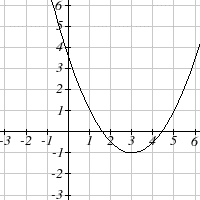
\includegraphics{images/image065.png
}
\caption{}
\end{figure}

The basic shape we will use is the rectangle; the area of a rectangle is
base\textbackslash{}( \textbackslash{}cdot \textbackslash{})height. You
should also know the area formulas for triangles, \textbackslash{}(
A=\textbackslash{}frac\{1\}\{2\}bh \textbackslash{}), and for circles,
\textbackslash{}( A=\textbackslash{}pi r\^{}2 \textbackslash{}).

\hypertarget{section-3.1-the-definite-integral}{%
\section{Section 3.1: The Definite
Integral}\label{section-3.1-the-definite-integral}}

\hypertarget{distance-from-velocity}{%
\subsection{Distance from Velocity}\label{distance-from-velocity}}

\hypertarget{example-1}{%
\paragraph{Example 1}\label{example-1}}

Suppose a car travels on a straight road at a constant speed of 40 miles
per hour for two hours. See the graph of its velocity below. How far has
it gone?

\begin{figure}
\centering
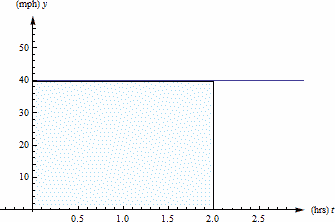
\includegraphics{images/image001.png}
\caption{}
\end{figure}

We all remember distance = rate\textbackslash{}( \textbackslash{}cdot
\textbackslash{})time, so this one is easy. The car has gone (40
miles/hour)\textbackslash{}( \textbackslash{}cdot \textbackslash{})(2
hours) = 80 miles.

\hypertarget{example-2}{%
\paragraph{Example 2}\label{example-2}}

Now suppose that a car travels so that its speed increases steadily from
0 to 40 miles per hour, for two hours. (Just be grateful you weren't
stuck behind this car on the highway.) See the graph of its velocity in
below. How far has this car gone?

\begin{figure}
\centering
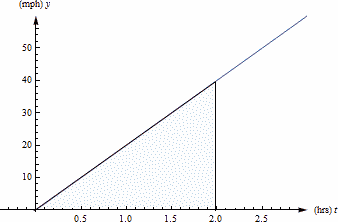
\includegraphics{images/image002.png}
\caption{}
\end{figure}

The trouble with our old reliable \textbf{distance =
rate\textbackslash{}( \textbackslash{}cdot \textbackslash{})time}
relationship is that it only works if the rate is constant. If the rate
is changing, there isn't a good way to use this formula.

But look at the graph from the last example again. Notice that
\textbf{distance = rate\textbackslash{}( \textbackslash{}cdot
\textbackslash{})time} also describes the area between the velocity
graph and the \textbackslash{}(t\textbackslash{})-axis, between
\textbackslash{}(t = 0\textbackslash{}) and \textbackslash{}(t =
2\textbackslash{}) hours. The \textbf{rate} is the height of the
rectangle, the \textbf{time} is the length of the rectangle, and the
\textbf{distance} is the \textbf{area} of the rectangle. This is the way
we can extend our simple formula to handle more complicated velocities:
And this is the way we can answer the second example.

The distance the car travels is the area between its velocity graph, the
\textbackslash{}(t\textbackslash{})-axis, \textbackslash{}(t =
0\textbackslash{}) and \textbackslash{}(t = 2\textbackslash{}). This
region is a triangle, so its area is
\textbackslash{}{[}\textbackslash{}frac\{1\}\{2\}bh =
\textbackslash{}frac\{1\}\{2\}(2 \textbackslash{}text\{ hours\})(40
\textbackslash{}text\{ miles per hour\}) = 40 \textbackslash{}text\{
miles\}.\textbackslash{}{]} So the car travels 40 miles during its
annoying trip.

In our distance/velocity examples, the function represented a
\textbf{rate} of travel (miles per hour), and the area represented the
\textbf{total} distance traveled. This principle works more generally:

For functions representing other \textbf{rates} such as the production
of a factory (bicycles per day), or the flow of water in a river
(gallons per minute) or traffic over a bridge (cars per minute), or the
spread of a disease (newly sick people per week), the area will still
represent the \textbf{total} amount of something.

\begin{figure}
\centering
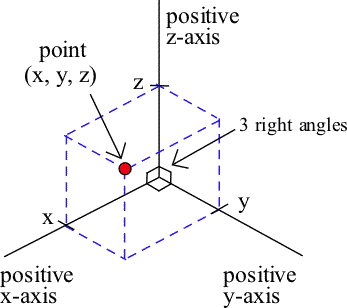
\includegraphics{images/image003.png}
\caption{}
\end{figure}

\hypertarget{example-3}{%
\paragraph{Example 3}\label{example-3}}

The graph below shows the flow rate (cubic feet per second) of water in
the Skykomish river at the town of Goldbar in Washington state.

\begin{figure}
\centering
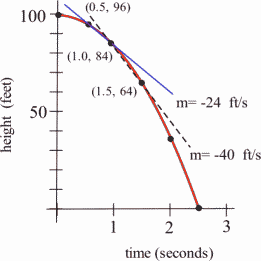
\includegraphics{images/image004.png}
\caption{}
\end{figure}

The area of the shaded region represents the total volume (cubic feet or
\textbackslash{}( \textbackslash{}text\{ft\}\^{}3 \textbackslash{})) of
water flowing past the town during the month of October. We can
approximate this area to approximate the total water by thinking of the
shaded region as a rectangle with a triangle on top.

\textbackslash{}{[} \textbackslash{}begin\{align*\}
\textbackslash{}text\{Total water \}=\& \textbackslash{}text\{ total
area\}\textbackslash{}\textbackslash{} \textbackslash{}approx\&
\textbackslash{}text\{ area of rectangle \}+\textbackslash{}text\{ area
of the "triangle"\} \textbackslash{}\textbackslash{}
\textbackslash{}approx\& \textbackslash{}left(2000
\textbackslash{}frac\{\textbackslash{}text\{ft\}\^{}3\}\{\textbackslash{}text\{s\}\}\textbackslash{}right)\textbackslash{}left(30
\textbackslash{}text\{
days\}\textbackslash{}right)+\textbackslash{}frac\{1\}\{2\}\textbackslash{}left(1500\textbackslash{}frac\{\textbackslash{}text\{ft\}\^{}3\}\{\textbackslash{}text\{s\}\}\textbackslash{}right)\textbackslash{}left(30\textbackslash{}text\{
days\}\textbackslash{}right) \textbackslash{}\textbackslash{} =\&
\textbackslash{}left(2570\textbackslash{}frac\{\textbackslash{}text\{ft\}\^{}3\}\{\textbackslash{}text\{s\}\}\textbackslash{}right)\textbackslash{}left(30\textbackslash{}text\{
days\}\textbackslash{}right) \textbackslash{}end\{align*\}
\textbackslash{}{]}

Note that we need to convert the units to make sense of our result:
\textbackslash{}{[} \textbackslash{}begin\{align*\}
\textbackslash{}text\{Total water \}\textbackslash{}approx\&
\textbackslash{}left(2570\textbackslash{}frac\{\textbackslash{}text\{ft\}\^{}3\}\{\textbackslash{}text\{s\}\}\textbackslash{}right)\textbackslash{}left(30\textbackslash{}text\{
days\}\textbackslash{}right) \textbackslash{}\textbackslash{} =\&
\textbackslash{}left(2570\textbackslash{}frac\{\textbackslash{}text\{ft\}\^{}3\}\{\textbackslash{}text\{s\}\}\textbackslash{}right)\textbackslash{}left(2,\textbackslash{}!592,\textbackslash{}!000\textbackslash{}text\{
sec\}\textbackslash{}right) \textbackslash{}\textbackslash{}
\textbackslash{}approx\& 7.128\textbackslash{}cdot
10\^{}9\textbackslash{}text\{ ft\}\^{}3 \textbackslash{}end\{align*\}
\textbackslash{}{]}

About 7 billion cubic feet of water flowed past Goldbar in October.

\hypertarget{approximating-with-rectangles}{%
\subsection{Approximating with
Rectangles}\label{approximating-with-rectangles}}

How do we approximate the area if the rate curve is, well, ``curvy''? We
could use rectangles and triangles, like we did in the last example. But
it turns out to be more useful (and easier) to simply use rectangles.
The more rectangles we use, the better our approximation is.

\begin{figure}
\centering
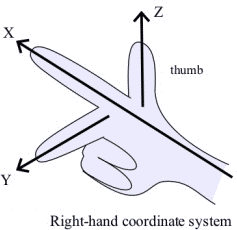
\includegraphics{images/image005.png}
\caption{}
\end{figure}

Suppose we want to calculate the area between the graph of a positive
function \textbackslash{}(f\textbackslash{}) and the
\textbackslash{}(x\textbackslash{})-axis on the interval
\textbackslash{}({[}a, b{]}\textbackslash{}) (graphed above). The
\textbf{Riemann Sum method} is to build several rectangles with bases on
the interval \textbackslash{}({[}a, b{]}\textbackslash{}) and sides that
reach up to the graph of \textbackslash{}(f\textbackslash{}) (see
below). Then the areas of the rectangles can be calculated and added
together to get a number called a Riemann Sum of
\textbackslash{}(f\textbackslash{}) on \textbackslash{}({[}a,
b{]}\textbackslash{}). The area of the region formed by the rectangles
is an \textbf{approximation} of the area we want.

\begin{figure}
\centering
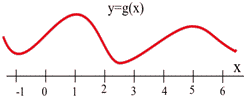
\includegraphics{images/image006.png}
\caption{}
\end{figure}

To view this video please enable JavaScript, and consider upgrading to a
web browser that \href{http://videojs.com/html5-video-support/}{supports
HTML5 video}

\hypertarget{example-4}{%
\paragraph{Example 4}\label{example-4}}

Approximate the area in the graph on the left between the graph of
\textbackslash{}(f\textbackslash{}) and the
\textbackslash{}(x\textbackslash{})-axis on the interval {[}2, 5{]} by
summing the areas of the rectangles in the graph on the right.

\begin{figure}
\centering
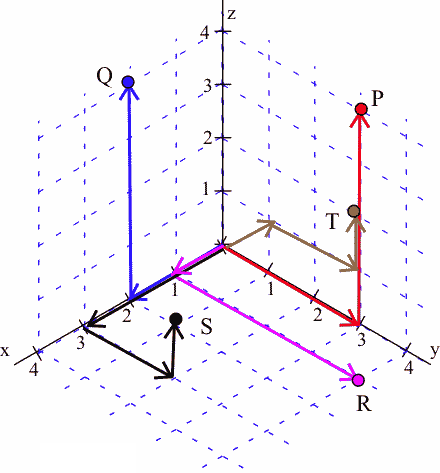
\includegraphics{images/image007.png}
\caption{}
\end{figure}

The total area of rectangles is \textbackslash{}{[}(2)(3) + (1)(5) =
11\textbackslash{}text\{ units\}\^{}2.\textbackslash{}{]}

\hypertarget{example-5}{%
\paragraph{Example 5}\label{example-5}}

Let \textbackslash{}(A\textbackslash{}) be the region bounded by the
graph of \textbackslash{}(f(x) =
\textbackslash{}frac\{1\}\{x\}\textbackslash{}), the
\textbackslash{}(x\textbackslash{})-axis, and vertical lines at
\textbackslash{}(x = 1\textbackslash{}) and \textbackslash{}(x =
5\textbackslash{}). We can't find the area exactly (with what we know
now), but we can approximate it using rectangles.

When we make our rectangles, we have a lot of choices. We could pick any
(non-overlapping) rectangles whose bottoms lie within the interval on
the x-axis, and whose tops intersect with the curve somewhere. But it is
easiest to choose rectangles that (a) have all the same width and (b)
take their heights from the function at one edge. Below are graphs
showing two ways to use four rectangles to approximate this area. In the
first graph, we used left-endpoints; the height of each rectangle comes
from the function value at its left edge. In the second graph on the
next page, we used right-hand endpoints.

\textbf{Left-hand endpoints:} The area is approximately the sum of the
areas of the rectangles. Each rectangle gets its height from the
function \textbackslash{}( f(x)=\textbackslash{}frac\{1\}\{x\}
\textbackslash{}) and each rectangle has a width of 1.

\begin{figure}
\centering
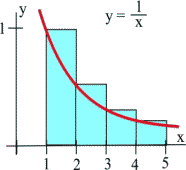
\includegraphics{images/image008.png}
\caption{}
\end{figure}

You can find the area of each rectangle using area =
height\textbackslash{}( \textbackslash{}cdot \textbackslash{})width. So
the total area of the rectangles, the left-hand estimate of the area
under the curve, is \textbackslash{}{[}f(1)\textbackslash{}cdot
1+f(2)\textbackslash{}cdot 1+f(3)\textbackslash{}cdot
1+f(4)\textbackslash{}cdot
1=1+\textbackslash{}frac\{1\}\{2\}+\textbackslash{}frac\{1\}\{3\}+\textbackslash{}frac\{1\}\{4\}=\textbackslash{}frac\{25\}\{12\}\textbackslash{}approx
2.08.\textbackslash{}{]}

Notice that because this function is decreasing, all the left endpoint
rectangles stick out above the region we want -- using left-hand
endpoints will overestimate the area.

\textbf{Right-hand endpoints:} The right-hand estimate of the area is
\textbackslash{}{[}f(2)\textbackslash{}cdot 1+f(3)\textbackslash{}cdot
1+f(4)\textbackslash{}cdot 1+f(5)\textbackslash{}cdot
1=\textbackslash{}frac\{1\}\{2\}+\textbackslash{}frac\{1\}\{3\}+\textbackslash{}frac\{1\}\{4\}+\textbackslash{}frac\{1\}\{5\}=\textbackslash{}frac\{77\}\{60\}\textbackslash{}approx
1.28.\textbackslash{}{]}

\begin{figure}
\centering
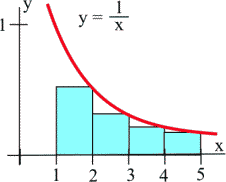
\includegraphics{images/image009.png}
\caption{}
\end{figure}

All the right-hand rectangles lie completely under the curve, so this
estimate will be an underestimate.

We can see that the true area is actually in between these two
estimates. So we could take their average:
\textbackslash{}{[}\textbackslash{}text\{Average\}=\textbackslash{}frac\{\textbackslash{}frac\{25\}\{12\}+\textbackslash{}frac\{77\}\{60\}\}\{2\}=\textbackslash{}frac\{101\}\{60\}\textbackslash{}approx
1.68\textbackslash{}{]}

In general, the average of the left-hand and right-hand estimates will
be closer to the real area than either individual estimate.

Our estimate of the area under the curve is about 1.68. (The actual area
is about 1.61.)

This applet will allow you to see how the approximation changes if you
use more rectangles; change the ``position'' slider to switch between
using the left endpoints, right endpoints, and midpoints:

To view this video please enable JavaScript, and consider upgrading to a
web browser that \href{http://videojs.com/html5-video-support/}{supports
HTML5 video}

If we wanted a better answer, we could use even more and even narrower
rectangles. But there is a limit to how much work we want to do by hand.
In practice, choose a manageable number of rectangles. We will have
better methods to get more accurate answers before long.

These sums of areas of rectangles are called \textbf{Riemann sums}. You
may see a shorthand notation used when people talk about sums. We won't
use it much in this book, but you should know what it means.

\hypertarget{riemann-sum}{%
\paragraph{Riemann Sum}\label{riemann-sum}}

A Riemann sum for a function \textbackslash{}(f(x)\textbackslash{}) over
an interval \textbackslash{}({[}a, b{]}\textbackslash{}) is a sum of
areas of rectangles that approximates the area under the curve. Start by
dividing the interval \textbackslash{}({[}a, b{]}\textbackslash{}) into
\textbackslash{}(n\textbackslash{}) subintervals; each subinterval will
be the base of one rectangle. We usually make all the rectangles the
same width \textbackslash{}( \textbackslash{}Delta x \textbackslash{}).
The height of each rectangle comes from the function evaluated at some
point in its sub interval. Then the Riemann sum is
\textbackslash{}{[}f(x\_1)\textbackslash{}Delta
x+f(x\_2)\textbackslash{}Delta x+f(x\_3)\textbackslash{}Delta
x+\textbackslash{}dots +f(x\_n)\textbackslash{}Delta
x\textbackslash{}{]} or, factoring out the \textbackslash{}(
\textbackslash{}Delta x \textbackslash{}),
\textbackslash{}{[}\textbackslash{}Delta
x\textbackslash{}left(f(x\_1)+f(x\_2)+f(x\_3)+\textbackslash{}dots
+f(x\_n)\textbackslash{}right).\textbackslash{}{]}

\hypertarget{sigma-notation}{%
\paragraph{Sigma Notation}\label{sigma-notation}}

The upper-case Greek letter Sigma \textbackslash{}( \textbackslash{}sum
\textbackslash{}) is used to stand for ``sum''. Sigma notation is a way
to compactly represent a sum of many similar terms, such as a Riemann
sum.

Using the Sigma notation, the Riemann sum can be written
\textbackslash{}{[}\textbackslash{}sum\textbackslash{}limits\_\{i=1\}\^{}n
f\textbackslash{}left(x\_i\textbackslash{}right)\textbackslash{}Delta
x.\textbackslash{}{]}

This is read aloud as ``the sum as \textbackslash{}(i\textbackslash{})
goes from 1 to \textbackslash{}(n\textbackslash{}) of
\textbackslash{}(f\textbackslash{}) of
\textbackslash{}(x\textbackslash{}) sub
\textbackslash{}(i\textbackslash{}) times Delta
\textbackslash{}(x\textbackslash{}).'' The
``\textbackslash{}(i\textbackslash{})'' is a counter or index, like you
might have seen in a programming class.

To view this video please enable JavaScript, and consider upgrading to a
web browser that \href{http://videojs.com/html5-video-support/}{supports
HTML5 video}

\hypertarget{definition-of-the-definite-integral}{%
\subsection{Definition of the Definite
Integral}\label{definition-of-the-definite-integral}}

Because the area under the curve is so important, it has a special
vocabulary and notation.

\hypertarget{the-definite-integral}{%
\paragraph{The Definite Integral}\label{the-definite-integral}}

The \textbf{definite integral} of a positive function
\textbackslash{}(f(x)\textbackslash{}) over an interval
\textbackslash{}({[}a, b{]}\textbackslash{}) is the area between
\textbackslash{}(f\textbackslash{}), the
\textbackslash{}(x\textbackslash{})-axis, \textbackslash{}(x =
a\textbackslash{}) and \textbackslash{}(x = b\textbackslash{}).

The \textbf{definite integral} of a positive function
\textbackslash{}(f(x)\textbackslash{}) from
\textbackslash{}(a\textbackslash{}) to
\textbackslash{}(b\textbackslash{}) is the area under the curve between
\textbackslash{}(a\textbackslash{}) and
\textbackslash{}(b\textbackslash{}).

If \textbackslash{}(f(t)\textbackslash{}) represents a positive rate (in
\textbackslash{}(y\textbackslash{})-units per
\textbackslash{}(t\textbackslash{})-units), then the definite integral
of \textbackslash{}(f(t)\textbackslash{}) from
\textbackslash{}(a\textbackslash{}) to
\textbackslash{}(b\textbackslash{}) is the total
\textbackslash{}(y\textbackslash{})-units that accumulate between
\textbackslash{}(t = a\textbackslash{}) and \textbackslash{}(t =
b\textbackslash{}).

\hypertarget{notation-for-the-definite-integral}{%
\subparagraph{Notation for the Definite
Integral}\label{notation-for-the-definite-integral}}

The definite integral of \textbackslash{}(f(x)\textbackslash{}) from
\textbackslash{}(a\textbackslash{}) to
\textbackslash{}(b\textbackslash{}) is written
\textbackslash{}{[}\textbackslash{}int\_a\^{}b f(x)\textbackslash{},
dx.\textbackslash{}{]}

The \textbackslash{}( \textbackslash{}int \textbackslash{}) symbol is
called the \textbf{integral sign}; it is an elongated letter S, standing
for ``sum''. (The \textbackslash{}( \textbackslash{}int
\textbackslash{}) corresponds to the \textbackslash{}(
\textbackslash{}sum \textbackslash{}) from the Riemann sum)

The \textbackslash{}(dx\textbackslash{}) on the end \emph{must} be
included! The \textbackslash{}(dx\textbackslash{}) tells what the
variable is -- in this example, the variable is
\textbackslash{}(x\textbackslash{}). (The
\textbackslash{}(dx\textbackslash{}) corresponds to the
\textbackslash{}( \textbackslash{}Delta x \textbackslash{}) from the
Riemann sum)

The function f is called the \textbf{integrand}.

The \textbackslash{}(a\textbackslash{}) and
\textbackslash{}(b\textbackslash{}) are called the \textbf{limits of
integration}.

\hypertarget{verb-forms}{%
\subparagraph{Verb forms}\label{verb-forms}}

We \textbf{integrate}, or \textbf{find the definite integral} of a
function. This process is called \textbf{integration}.

\hypertarget{formal-algebraic-definition}{%
\subparagraph{Formal Algebraic
Definition}\label{formal-algebraic-definition}}

\textbackslash{}{[}\textbackslash{}int\_a\^{}b f(x)\textbackslash{}, dx
=\textbackslash{}lim\textbackslash{}limits\_\{n\textbackslash{}to\textbackslash{}infty\}\textbackslash{}sum\textbackslash{}limits\_\{i=1\}\^{}n
f(x\_i)\textbackslash{}Delta x.\textbackslash{}{]}

\hypertarget{practical-definition}{%
\subparagraph{Practical Definition}\label{practical-definition}}

The definite integral can be approximated with a Riemann sum (dividing
the area into rectangles where the height of each rectangle comes from
the function, computing the area of each rectangle, and adding them up).
The more rectangles we use, the narrower the rectangles are, the better
our approximation will be.

\hypertarget{looking-ahead}{%
\subparagraph{Looking Ahead}\label{looking-ahead}}

We will have methods for computing exact values of some definite
integrals from formulas soon. In many cases, including when the function
is given to you as a table or graph, you will still need to approximate
the definite integral with rectangles.

\hypertarget{example-6}{%
\paragraph{Example 6}\label{example-6}}

The graph below shows \textbackslash{}(y = r(t)\textbackslash{}), the
number of telephone calls made per hours on a Tuesday. Approximately how
many calls were made between 9 pm and 11 pm? Express this as a definite
integral and approximate with a Riemann sum.

\begin{figure}
\centering
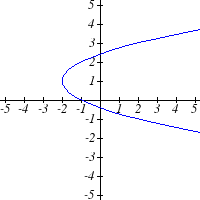
\includegraphics{images/image010.png}
\caption{}
\end{figure}

We know that the accumulated calls will be the area under this rate
graph over that two-hour period, the definite integral of this rate from
\textbackslash{}(t = 9\textbackslash{}) to \textbackslash{}(t =
11\textbackslash{}).

The total number of calls will be \textbackslash{}(
\textbackslash{}int\textbackslash{}limits\_9\^{}\{11\}
r(t)\textbackslash{},dt \textbackslash{}).

The top here is a curve, so we can't get an exact answer. But we can
approximate the area using rectangles. Let's choose to use four
rectangles and left-endpoints:

\begin{figure}
\centering
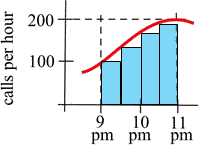
\includegraphics{images/image066.png}
\caption{}
\end{figure}

\textbackslash{}{[}\textbackslash{}int\textbackslash{}limits\_9\^{}\{11\}
r(t)\textbackslash{},dt \textbackslash{}approx
0.5(100+150+180+195)=312.5\textbackslash{}{]}

The units are calls per hour\textbackslash{}( \textbackslash{}cdot
\textbackslash{})hours = calls. Our estimate is that about 312 calls
were made between 9 pm and 11 pm. Is this an under-estimate or an
over-estimate?

\hypertarget{example-7}{%
\paragraph{Example 7}\label{example-7}}

Describe the area between the graph of \textbackslash{}(f(x) =
\textbackslash{}frac\{1\}\{x\}\textbackslash{}), the
\textbackslash{}(x\textbackslash{})-axis, and the vertical lines at
\textbackslash{}(x = 1\textbackslash{}) and \textbackslash{}(x =
5\textbackslash{}) as a definite integral.

This is the same area we estimated to be about 1.68 before. Now we can
use the notation of the definite integral to describe it. Our estimate
of \textbackslash{}( \textbackslash{}int\textbackslash{}limits\_1\^{}5
\textbackslash{}frac\{1\}\{x\}\textbackslash{}, dx \textbackslash{}) was
1.68. The true value of \textbackslash{}(
\textbackslash{}int\textbackslash{}limits\_1\^{}5
\textbackslash{}frac\{1\}\{x\}\textbackslash{}, dx \textbackslash{}) is
about 1.61.

\hypertarget{example-8}{%
\paragraph{Example 8}\label{example-8}}

Using the idea of area, determine the value of \textbackslash{}(
\textbackslash{}int\textbackslash{}limits\_1\^{}3 1+x
\textbackslash{},dx \textbackslash{}).

\textbackslash{}( \textbackslash{}int\textbackslash{}limits\_1\^{}3 1+x
\textbackslash{},dx \textbackslash{}) represents the area between the
graph of \textbackslash{}(f(x) = 1+x\textbackslash{}), the
\textbackslash{}(x\textbackslash{})-axis, and the vertical lines at 1
and 3.

\begin{figure}
\centering
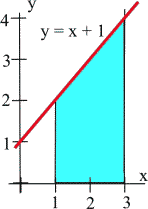
\includegraphics{images/image011.png
}
\caption{}
\end{figure}

Since this area can be broken into a rectangle and a triangle, we can
find the area exactly. The area equals \textbackslash{}{[} 4 +
\textbackslash{}frac\{1\}\{2\}(2)(2) = 6 \textbackslash{}text\{
units\}\^{}2.\textbackslash{}{]}

\hypertarget{example-9}{%
\paragraph{Example 9}\label{example-9}}

The table shows rates of population growth for Berrytown for several
years. Use this table to estimate the total population growth from 1970
to 2000:

\begin{longtable}[]{@{}lllll@{}}
\toprule
\endhead
Year, \textbackslash{}( t \textbackslash{}) & 1970 & 1980 & 1990 &
2000\tabularnewline
Rate of population growth \textbackslash{}( R(t) \textbackslash{}) in
thousands of people per year & 1.5 & 1.9 & 2.2 & 2.4\tabularnewline
\bottomrule
\end{longtable}

The definite integral of this rate will give the total change in
population over the thirty-year period. We only have a few pieces of
information, so we can only estimate. Even though we haven't made a
graph, we're still approximating the area under the rate curve, using
rectangles. How wide are the rectangles? We have information every 10
years, so the rectangles have a width of 10 years. How many rectangles?
Be careful here -- this is a thirty-year span, so there are three
rectangles.

\begin{itemize}
\tightlist
\item
  Using left-hand endpoints: (1.5)(10) + (1.9)(10) + (2.2)(10) = 56
\item
  Using right-hand endpoints: (1.9)(10) + (2.2)(10) + (2.4)(10) = 65
\end{itemize}

Taking the average of these two:
\textbackslash{}{[}\textbackslash{}frac\{56+65\}\{2\}=60.5\textbackslash{}{]}

Our best estimate of the total population growth from 1970 to 2000 is
\textbf{60.5 thousand people}.

To view this video please enable JavaScript, and consider upgrading to a
web browser that \href{http://videojs.com/html5-video-support/}{supports
HTML5 video}

\hypertarget{signed-area}{%
\subsection{Signed Area}\label{signed-area}}

You may have noticed that until this point, we've insisted that the
integrand (the function we're integrating) be positive. That's because
we've been talking about area, which is always positive.

If the ``height'' (from the function) is a negative number, then
multiplying it by the width doesn't give us actual area, it gives us the
area with a negative sign.

But it turns out to be useful to think about the possibility of negative
area. We'll expand our idea of a definite integral now to include
integrands that might not always be positive. The ``heights'' of the
rectangles, the values from the function, now might not always be
positive.

\hypertarget{the-definite-integral-and-signed-area}{%
\paragraph{The Definite Integral and Signed
Area}\label{the-definite-integral-and-signed-area}}

The \textbf{definite integral} of a function
\textbackslash{}(f(x)\textbackslash{}) over an interval
\textbackslash{}({[}a, b{]}\textbackslash{}) is the \textbf{signed area}
between \textbackslash{}(f\textbackslash{}), the
\textbackslash{}(x\textbackslash{})-axis, \textbackslash{}(x =
a\textbackslash{}) and \textbackslash{}(x = b\textbackslash{}).

The \textbf{definite integral} of a function
\textbackslash{}(f(x)\textbackslash{}) from
\textbackslash{}(a\textbackslash{}) to
\textbackslash{}(b\textbackslash{}) is the \textbf{signed area} under
the curve between \textbackslash{}(a\textbackslash{}) and
\textbackslash{}(b\textbackslash{}).

If the function is positive, the signed area is positive, as before (and
we can call it area.)

If the function dips below the \textbackslash{}(x\textbackslash{})-axis,
the areas of the regions below the
\textbackslash{}(x\textbackslash{})-axis come in with a negative sign.
In this case, we cannot call it simply ``area.'' These negative areas
take away from the definite integral.

\textbackslash{}( \textbackslash{}int\textbackslash{}limits\_a\^{}b f(x)
\textbackslash{},dx = \textbackslash{}) (Area above \textbackslash{}( x
\textbackslash{})-axis) \textbackslash{}( - \textbackslash{}) (Area
below \textbackslash{}( x \textbackslash{})-axis)

If f(t) represents a positive rate (in
\textbackslash{}(y\textbackslash{})-units per
\textbackslash{}(t\textbackslash{})-units), then the \textbf{definite
integral} of \textbackslash{}(f\textbackslash{}) from
\textbackslash{}(a\textbackslash{}) to
\textbackslash{}(b\textbackslash{}) is the \textbf{total}
\textbackslash{}(y\textbackslash{})-units that accumulate between
\textbackslash{}(t = a\textbackslash{}) and \textbackslash{}(t =
b\textbackslash{}).

If \textbackslash{}(f(t)\textbackslash{}) represents any rate (in
\textbackslash{}(y\textbackslash{})-units per
\textbackslash{}(t\textbackslash{})-units), then the \textbf{definite
integral} of \textbackslash{}(f\textbackslash{}) from
\textbackslash{}(a\textbackslash{}) to
\textbackslash{}(b\textbackslash{}) is the \textbf{net}
\textbackslash{}(y\textbackslash{})-units that accumulate between
\textbackslash{}(t = a\textbackslash{}) and \textbackslash{}(t =
b\textbackslash{}).

\hypertarget{example-10}{%
\paragraph{Example 10}\label{example-10}}

Find the definite integral of \textbackslash{}(f(x) =
--2\textbackslash{}) on the interval {[}1,4{]}.

\begin{figure}
\centering
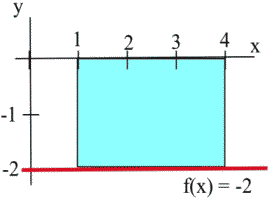
\includegraphics{images/image012.png}
\caption{}
\end{figure}

\textbackslash{}(\textbackslash{}int\textbackslash{}limits\_1\^{}4
-2\textbackslash{},dx\textbackslash{}) is the signed area of the region
shown to the right. The region lies below the \textbackslash{}( x
\textbackslash{})-axis, so the area, 6, comes in with a negative sign.
So the definite integral is
\textbackslash{}(\textbackslash{}int\textbackslash{}limits\_1\^{}4
-2\textbackslash{},dx =-6\textbackslash{}).

Negative rates indicate that the amount is decreasing. For example, if
\textbackslash{}(f(t)\textbackslash{}) is the velocity of a car in the
positive direction along a straight line at time
\textbackslash{}(t\textbackslash{}) (miles/hour), then negative values
of \textbackslash{}(f\textbackslash{}) indicate that the car is
traveling in the negative direction, backwards. The definite integral of
\textbackslash{}(f\textbackslash{}) is the change in position of the car
during the time interval. If the velocity is positive, positive distance
accumulates. If the velocity is negative, distance in the negative
direction accumulates.

This is true of any rate. For example, if
\textbackslash{}(f(t)\textbackslash{}) is the rate of population change
(people/year) for a town, then negative values of
\textbackslash{}(f\textbackslash{}) would indicate that the population
of the town was getting smaller, and the definite integral (now a
negative number) would be the \textbf{change} in the population, a
decrease, during the time interval.

\hypertarget{example-11}{%
\paragraph{Example 11}\label{example-11}}

In 1980 there were 12,000 ducks nesting around a lake, and the rate of
population change (in ducks per year) is shown in the figure below.
Write a definite integral to represent the total change in the duck
population from 1980 to 1990, and estimate the population in 1990.

\begin{figure}
\centering
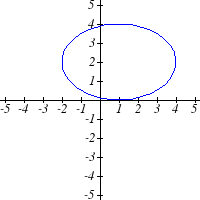
\includegraphics{images/image013.png}
\caption{}
\end{figure}

The change in population is: \textbackslash{}{[}
\textbackslash{}begin\{align*\}
\textbackslash{}int\textbackslash{}limits\_\{1980\}\^{}\{1990\} f(t)
\textbackslash{},dt=\& -(\textbackslash{}text\{area between
\textbackslash{}( f \textbackslash{}) and axis\})
\textbackslash{}\textbackslash{} \textbackslash{}approx\&
-(200\textbackslash{}text\{ ducks/year\})\textbackslash{}cdot
(10\textbackslash{}text\{ years\}) \textbackslash{}\textbackslash{} =\&
-2000\textbackslash{}text\{ ducks\} \textbackslash{}end\{align*\}
\textbackslash{}{]}

Then (1990 duck population) = (1980 population) + (change from 1980 to
1990) = (12,000) + ( -2000) = 10,000 ducks.

To view this video please enable JavaScript, and consider upgrading to a
web browser that \href{http://videojs.com/html5-video-support/}{supports
HTML5 video}

\hypertarget{example-12}{%
\paragraph{Example 12}\label{example-12}}

A bug starts at the location \textbackslash{}(x = 12\textbackslash{}) on
the \textbackslash{}(x\textbackslash{})-axis at 1 pm walks along the
axis with the velocity \textbackslash{}(v(x)\textbackslash{}) shown in
the graph. How far does the bug travel between 1 pm and 3 pm, and where
is the bug at 3 pm?

\begin{figure}
\centering
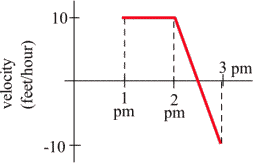
\includegraphics{images/image014.png}
\caption{}
\end{figure}

Note that the velocity is positive from 1 until 2:30, then becomes
negative. So the bug moves in the positive direction from 1 until 2:30,
then turns around and moves back toward where it started. The area under
the velocity curve from 1 to 2:30 shows the total distance traveled by
the bug in the positive direction; the bug moved 12.5 feet in the
positive direction. The \textbf{area} between the velocity curve and the
x-axis, between 2:30 and 3, shows the total distance traveled by the bug
in the negative direction, back toward home; the bug traveled 2.5 feet
in the negative direction. The definite integral of the velocity curve,
\textbackslash{}(\textbackslash{}int\textbackslash{}limits\_1\^{}3 v(t)
\textbackslash{},dt\textbackslash{}), shows the net change in distance:
\textbackslash{}{[}\textbackslash{}int\textbackslash{}limits\_1\^{}3
v(t) \textbackslash{},dt = 12.5-2.5=10.\textbackslash{}{]}

The bug ended up 10 feet farther in the positive direction than he
started. At 3 pm, the bug is at \textbackslash{}(x =
22\textbackslash{}).

\hypertarget{example-13}{%
\paragraph{Example 13}\label{example-13}}

Use the graph below to calculate \textbackslash{}(
\textbackslash{}int\textbackslash{}limits\_0\^{}2 f(x)
\textbackslash{},dx \textbackslash{}), \textbackslash{}(
\textbackslash{}int\textbackslash{}limits\_2\^{}4 f(x)
\textbackslash{},dx \textbackslash{}), \textbackslash{}(
\textbackslash{}int\textbackslash{}limits\_4\^{}5 f(x)
\textbackslash{},dx \textbackslash{}), and \textbackslash{}(
\textbackslash{}int\textbackslash{}limits\_0\^{}5 f(x)
\textbackslash{},dx \textbackslash{}).

\begin{figure}
\centering
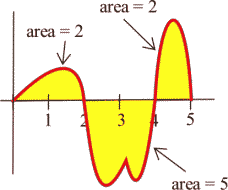
\includegraphics{images/image015.png}
\caption{}
\end{figure}

Using the given areas, \textbackslash{}(
\textbackslash{}int\textbackslash{}limits\_0\^{}2 f(x)
\textbackslash{},dx = 2 \textbackslash{}), \textbackslash{}(
\textbackslash{}int\textbackslash{}limits\_2\^{}4 f(x)
\textbackslash{},dx = -5 \textbackslash{}), \textbackslash{}(
\textbackslash{}int\textbackslash{}limits\_4\^{}5 f(x)
\textbackslash{},dx = 2 \textbackslash{}), and \textbackslash{}(
\textbackslash{}int\textbackslash{}limits\_0\^{}5 f(x)
\textbackslash{},dx = \textbackslash{})(area above)\textbackslash{}( -
\textbackslash{})(area below)\textbackslash{}( = (2+2) - (5) =
-1\textbackslash{}).

\hypertarget{approximating-with-technology}{%
\subsection{Approximating with
Technology}\label{approximating-with-technology}}

If your function is given as a graph or table, you will still have to
approximate definite integrals using areas, usually of rectangles. But
if your function is given as a formula, you can turn to technology to
get a better approximate answer. For example, most graphing calculators
have some kind of numerical integration tool built in. You can also find
many online tools that can do this; type numerical integration into any
search engine to see a selection of these.

Most numerical integration tools use rectangles to estimate the signed
area, just as you would do by hand. But they use many more rectangles
than you would have the patience for, so they get a better answer. Some
of them use computer algebra systems to find exact answers; we will
learn how to do this ourselves later in this chapter.

When you turn to technology to find the value of a definite integral, be
careful. Not every tool will be able to give you a correct answer for
every integral. You should make an estimate of the answer yourself first
so you can judge whether the answer you get makes sense.

\hypertarget{example-14}{%
\paragraph{Example 14}\label{example-14}}

Use technology to approximate the definite integral \textbackslash{}(
\textbackslash{}int\textbackslash{}limits\_1\^{}5
\textbackslash{}frac\{1\}\{x\} \textbackslash{},dx \textbackslash{}).
(This is the same definite integral we approximated with rectangles
before.)

We could use the following command in GeoGebra to approximate this
integral:

\texttt{Integral{[}1\ /\ x,\ 1,\ 5{]}}

Or
\href{http://www.wolframalpha.com/input/?i=integrate+1\%2Fx+from+1+to+5}{click
this link} to see how to evaluate this integral using
\href{http://www.wolframalpha.com/}{Wolfram\textbar{}Alpha}.

\hypertarget{example-15}{%
\paragraph{Example 15}\label{example-15}}

Use technology to approximate the definite integral \textbackslash{}(
\textbackslash{}int\textbackslash{}limits\_1\^{}2 e\^{}\{x\^{}2+x\}
\textbackslash{},dx \textbackslash{}).

The function here is positive, so there must be some area under the
curve here. There isn't an algebraic way to find the exact answer, so
some programs may just return the original integral rather than try to
approximate it.

We could use the following command in GeoGebra to approximate this
integral:

\texttt{Integral{[}e\^{}(x\^{}2\ +\ x),\ 1,\ 2{]}}

Or
\href{http://www.wolframalpha.com/input/?i=integrate+e\%5E(x\%5E2\%2Bx)+from+1+to+2}{click
this link} to see how to approximate this integral using
\href{http://www.wolframalpha.com/}{Wolfram\textbar{}Alpha}. Although it
looks like Wolfram\textbar{}Alpha can evaluate the integral, the
``Erfi'' function that it shows in its answer is actually defined in
terms of another integral, so it still hasn't found an algebraic answer.

\hypertarget{accumulation-in-real-life}{%
\subsection{Accumulation in Real Life}\label{accumulation-in-real-life}}

We have already seen that the ``area'' under a graph can represent
quantities whose units are not the usual geometric units of square
meters or square feet. For example, if
\textbackslash{}(t\textbackslash{}) is a measure of time in seconds and
\textbackslash{}(f(t)\textbackslash{}) is a velocity with units
feet/second, then the definite integral has units
(feet/second)\textbackslash{}( \textbackslash{}cdot
\textbackslash{})(seconds) = feet.

In general, the units for the definite integral \textbackslash{}(
\textbackslash{}int\textbackslash{}limits\_a\^{}b
f(x)\textbackslash{},dx \textbackslash{}) are
(\textbackslash{}(y\textbackslash{})-units )\textbackslash{}(
\textbackslash{}cdot
\textbackslash{})(\textbackslash{}(x\textbackslash{})-units). A quick
check of the units can help avoid errors in setting up an applied
problem.

In previous examples, we looked at a function that represented a
\textbf{rate} of travel (miles per hour); in that case, the area
represented the \textbf{total} distance traveled. For functions
representing other \textbf{rates} such as the production of a factory
(bicycles per day), or the flow of water in a river (gallons per minute)
or traffic over a bridge (cars per minute), or the spread of a disease
(newly sick people per week), the area will still represent the
\textbf{total} amount of something.

\hypertarget{example-16}{%
\paragraph{Example 16}\label{example-16}}

Suppose \textbackslash{}(MR(q)\textbackslash{}) is the marginal revenue
in dollars/item for selling \textbackslash{}(q\textbackslash{}) items.
What does \textbackslash{}(
\textbackslash{}int\textbackslash{}limits\_0\^{}\{150\} MR(q)
\textbackslash{},dq \textbackslash{}) represent?

\textbackslash{}(
\textbackslash{}int\textbackslash{}limits\_0\^{}\{150\} MR(q)
\textbackslash{},dq \textbackslash{}) has units
(dollars/item)\textbackslash{}( \textbackslash{}cdot
\textbackslash{})(items) = dollars, and represents the accumulated
dollars for selling from 0 to 150 items. That is, \textbackslash{}(
\textbackslash{}int\textbackslash{}limits\_0\^{}\{150\} MR(q)
\textbackslash{},dq = TR(150) \textbackslash{}), the total revenue from
selling 150 items.

\hypertarget{example-17}{%
\paragraph{Example 17}\label{example-17}}

Suppose \textbackslash{}(r(t)\textbackslash{}), in centimeters per year,
represents how the diameter of a tree changes with time. What does
\textbackslash{}(
\textbackslash{}int\textbackslash{}limits\_\{T\_1\}\^{}\{T\_2\} r(t)
\textbackslash{},dt \textbackslash{}) represent?

\textbackslash{}(
\textbackslash{}int\textbackslash{}limits\_\{T\_1\}\^{}\{T\_2\} r(t)
\textbackslash{},dt \textbackslash{}) has units of (centimeters per
year)\textbackslash{}( \textbackslash{}cdot \textbackslash{})(years) =
centimeters, and represents the accumulated growth of the tree's
diameter from \textbackslash{}(T\_1\textbackslash{}) to
\textbackslash{}(T\_2\textbackslash{}). That is, \textbackslash{}(
\textbackslash{}int\textbackslash{}limits\_\{T\_1\}\^{}\{T\_2\} r(t)
\textbackslash{},dt \textbackslash{}) is the change in the diameter of
the tree over this period of time.

\begin{longtable}[]{@{}ll@{}}
\toprule
\endhead
\href{../chapter2/section2-11.php}{← Previous Section} &
\href{section3-2.php}{Next Section →}\tabularnewline
\bottomrule
\end{longtable}
